\section{Μεγάλη Ακολουθία}

Ο αλγόριθμος που υλοποιήθηκε για την παραγωγή της μεγάλης ακολουθίας βασίζεται σε μία απλούστερη συλλογιστική.
Αυτή τη φορά ο αλγόριθμος εφαρμόστηκε σε ολόκληρο το σύνολο δεδομένων και δεν πραγματοποιήθηκε καμία επιλογή εταιρειών με οποιονδήποτε τρόπο.

Γνωρίζοντας πλέον ότι το μέγιστο επιτρεπτό πλήθος συναλλαγών είναι πολύ μεγαλύτερο από το πλήθος των ημερών του συνόλου δεδομένων μας, μπορούμε να περιορίσουμε το χρονικό παράθυρο σε μία μόνο ημέρα, και μάλιστα να πραγματοποιήσουμε πολλαπλές συναλλαγές ανά ημέρα.

Εκμεταλλευόμαστε λοιπόν το ``intra-day trading'', όπως αυτό περιγράφεται από την εκφώνηση της άσκησης, και εφαρμόζουμε μία αντίστοιχα άπληστη λογική με αυτήν που περιγράφθηκε στην προηγούμενη ενότητα.
Επικεντρωνόμαστε σε δύο είδη ομάδων συναλλαγών:
\begin{itemize}
    \item Αγορά στην τιμή ανοίγματος της μετοχής και πώληση στη μέγιστη καταγραφείσα τιμή της, και
    \item Αγορά στην χαμηλότερη καταγραφείσα τιμή της μετοχής και πώληση στην τιμή κλεισίματός της.
\end{itemize}

Κάθε ημέρα λαμβάνουν χώρα συναλλαγές μόνο της μίας εκ των δύο αυτών ομάδων.
Ωστόσο, για την επιλογή μίας εκ των δύο, υπολογίζεται το κέρδος και των δύο αυτών περιπτώσεων.
Για την ακρίβεια, κάθε ημέρα χωρίζουμε τις εταιρείες σε δύο ομάδες με κριτήριο την περίπτωση (μεταξύ των προαναφερθέντων δύο) στην οποία μεγιστοποιείται το κέρδος από την αγοραπωλησία τους, εφόσον η αγοραπωλησία τους μπορεί να είναι επικερδής.
Στην συνέχεια, μετά την κατάλληλη σταχυολόγησή τους με τρόπο παρόμοιο με αυτόν που περιγράφθηκε για τον αλγόριθμο παραγωγής της μικρής ακολουθίας, υπολογίζουμε ποιας ομάδας εναπομεινασών εταιρειών η αγοραπωλησία μπορεί να αποφέρει μεγαλύτερο κέρδος, και επιλέγουμε άπληστα την βέλτιστη εκ των δύο.
Μία εύκολη βελτιστοποίηση του αλγορίθμου που θα μπορούσε να γίνει στο σημείο αυτό είναι η επιπρόσθετη αγορά μετοχών και των υπόλοιπων εταιρειών (της άλλης ομάδας), βέβαια μόνο εφόσον παραμένουν επικερδείς και στην περίπτωση του έτερου intra-day trading παραθύρου.

Παρ'ολ'αυτά, δεν χρειάστηκε να υλοποιηθούν και να εφαρμοστούν περαιτέρω βελτιστοποιήσεις στον αλγόριθμο, διότι το κέρδος που επετεύχθη αποδεικνύεται αρκούντως ικανοποιητικό για τον παρεχόμενο online επικυρωτή, σύμφωνα με τον οποίον η ακολουθία που παράχθηκε αποφέρει κέρδος $67974244180.00747$ ($\approx \num{6.8e10}$) δολλαρίων κατόπιν $314164$ συναλλαγών.

Παρατηρούμε ότι παρότι το πλήθος των συναλλαγών είναι αρκετών τάξεων μεγέθους μεγαλύτερο από το αντίστοιχο της περίπτωσης της παραγωγής της μικρής ακολουθίας της προηγούμενης ενότητας, εν τέλει το κέρδος δεν είναι αντίστοιχα αυξημένο κατά πολλές τάξεις μεγέθους.
Η βασική αιτία που εξηγεί αυτή την συμπεριφορά είναι βέβαια η φύση του αλγορίθμου που υλοποιήθηκε.

Επιβάλλοντας την άπληστη αγοραπωλησία μετοχών των εταιρειών σε ημερήσια βάση, χάνονται πολλές ενδεχόμενες μεγάλες αυξήσεις τιμών μετοχών εταιρειών μεταξύ πολλαπλών ημερών -- περιπτώσεις τις οποίες ο αλγόριθμος που υλοποιήθηκε για τον υπολογισμό της μικρής ακολουθίας θα εντόπιζε επιτυχώς και θα εκμεταλλευόταν.
Συν τοις άλλοις, για την περίπτωση του υπολογισμού της μεγάλης ακολουθίας καταβλήθηκε συνολικά σημαντικά λιγότερη προσπάθεια στην βελτιστοποίηση του ίδιου του αλγορίθμου, ακριβώς διότι υπήρχε η γνώση ότι το αρκετά μεγαλύτερο επιτρεπτό πλήθος συναλλαγών θα μπορούσε να οδηγήσει σε αποδεκτές λύσεις οι οποίες θα μπορούσαν να βασίζονται σε λιγότερο σύνθετη συλλογιστική.

Το αντίστοιχο διάγραμμα αποτίμησης της περίπτωσης της μεγάλης ακολουθίας παρατίθεται στο παρακάτω σχήμα.
Παρατηρούμε ότι αυτή την φορά στο κλείσιμο κάθε ημέρας δεν υπάρχει καμία μετοχή εταιρείας στην κατοχή μας, αφού ο αλγόριθμος ορίζει ότι πρέπει να έχουν όλες πωληθεί μέχρι το τέλος κάθε ημέρας.
Επομένως, το διάγραμμα αποτίμησης έχει πρακτικά εκφυλιστεί σε διάγραμμα του υπολοίπου του λογαριασμού.

\begin{figure}[H]
\centering
%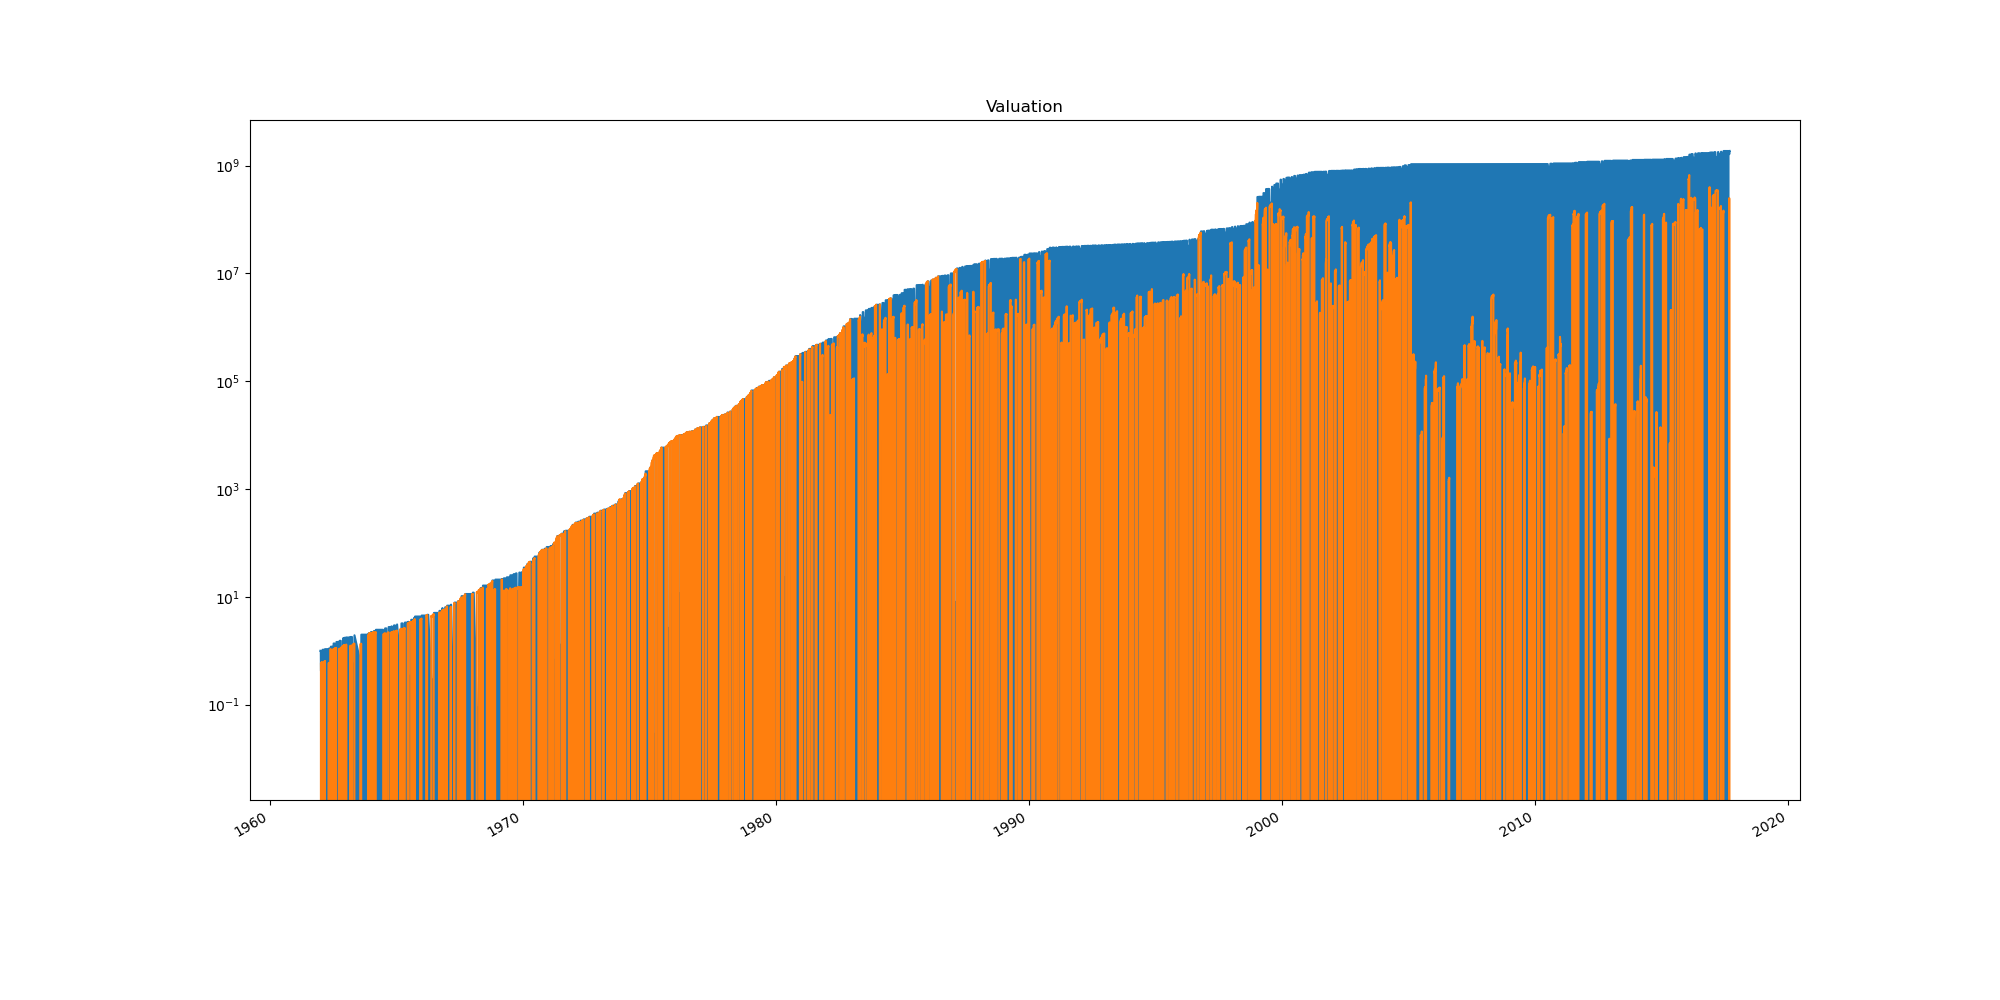
\includegraphics[scale=0.4]{images/small.png}
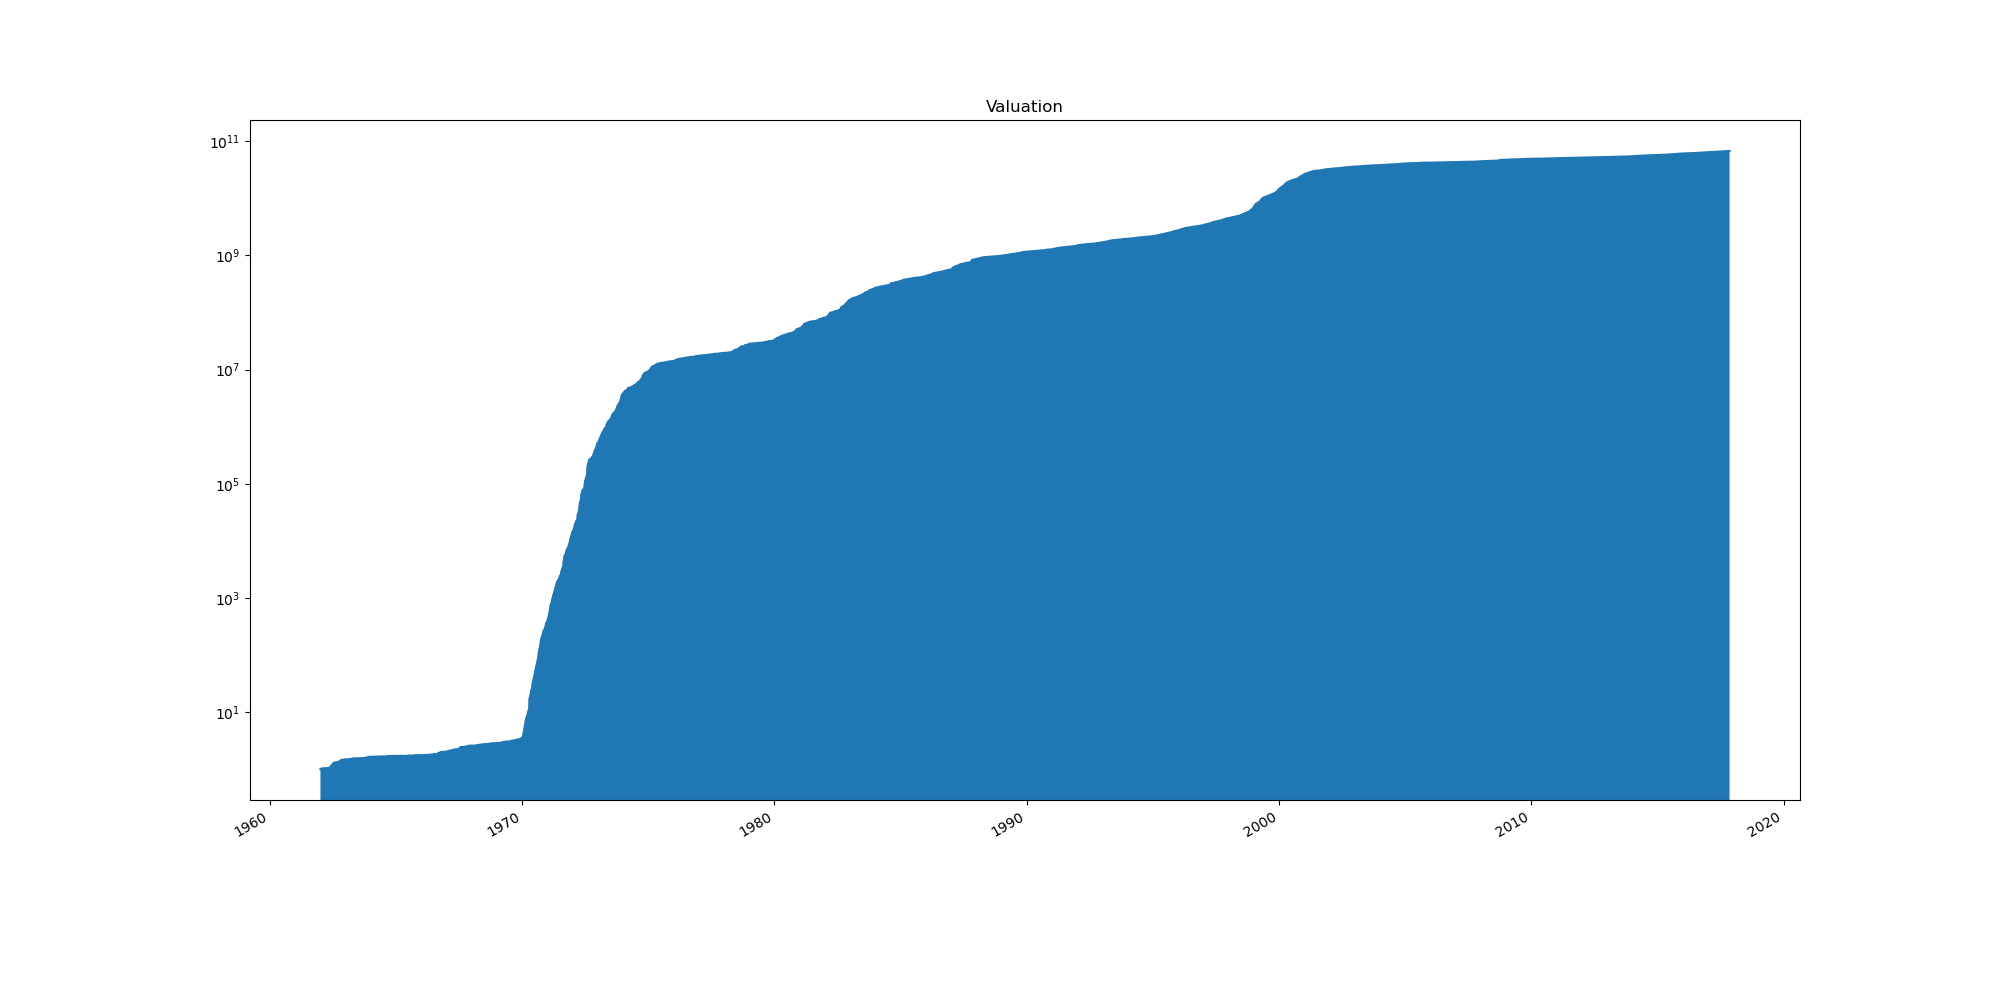
\includegraphics[width=1.1\linewidth]{images/large.png}
\captionof{figure}{Διάγραμμα αποτίμησης κατά τον υπολογισμό της μεγάλης ακολουθίας.}
\label{fig:valuation_large}
\end{figure}

Μία άλλη παρατήρηση που αξίζει να σημειωθεί είναι ότι, και πάλι λόγω της φύσης του παρόντος αλγορίθμου σε σχέση με αυτού της προηγούμενης ενότητας, το προκείμενο διάγραμμα αποτίμησης ``ακολουθεί'' καλύτερα την ευρύτερη τάση του χρηματιστηρίου (εφόσον η πώληση κάθε μετοχής πραγματοποιείται την ημέρα της αγοράς της), σε αντίθεση με το αντίστοιχο διάγραμμα της προηγούμενης ενότητας, το οποίο χρησιμοποιούσε το χρονικό παράθυρο ``αλλοιώνοντας'' έτσι την αντίστοιχη απεικόνιση της τάσης του χρηματιστηρίου σε επίπεδο ευαισθησίας $40$ ημερών.
